\documentclass{beamer}
\usetheme{CambridgeUS}
\usecolortheme{default}
\setbeamercolor{itemize item}{fg=darkred!80!black}

\makeatletter
\setbeamertemplate{footline}
{
  \leavevmode%
  \hbox{%
  \begin{beamercolorbox}[wd=.333333\paperwidth,ht=2.25ex,dp=1ex,center]{author in head/foot}%
    \usebeamerfont{author in head/foot}F. Massa
  \end{beamercolorbox}%
  \begin{beamercolorbox}[wd=.333333\paperwidth,ht=2.25ex,dp=1ex,center]{title in head/foot}%
    \usebeamerfont{title in head/foot}Supervisors: G. Chiarelli, C. Gemme
  \end{beamercolorbox}%
  \begin{beamercolorbox}[wd=.333333\paperwidth,ht=2.25ex,dp=1ex,right]{date in head/foot}%
    \usebeamerfont{date in head/foot}\insertshortdate{}\hspace*{2em}
    \insertframenumber{} / \inserttotalframenumber\hspace*{2ex} 
  \end{beamercolorbox}}%
  \vskip0pt%
}
\makeatother

\title{ITk performances in the
$H \rightarrow ZZ^{*} \rightarrow 4\mu$ channel \\
with a fast sim method}
%\subtitle{Subtitle}
\author{Federico Massa}
\institute{ITk Simulation \& Performance}
\date{Sept. 7, 2016}

\usepackage[export]{adjustbox}
\usepackage{tikz}
\usetikzlibrary{decorations.pathreplacing,calc}
\newcommand{\tikzmark}[1]{\tikz[overlay,remember picture] \node (#1) {};}

\usepackage{xcolor}
\definecolor{dred}{RGB}{200,0,0}

\usepackage[font=small,skip=0pt]{caption}
\usepackage{textcomp}

\setbeamertemplate{navigation symbols}{}
\begin{document}

\begin{frame}
\titlepage
\end{frame}

%----------------------------------------------

\begin{frame}
\frametitle{The Fast Sim method - RoI definition}

\begin{columns}[t]
	\begin{column}{.7\textwidth}
		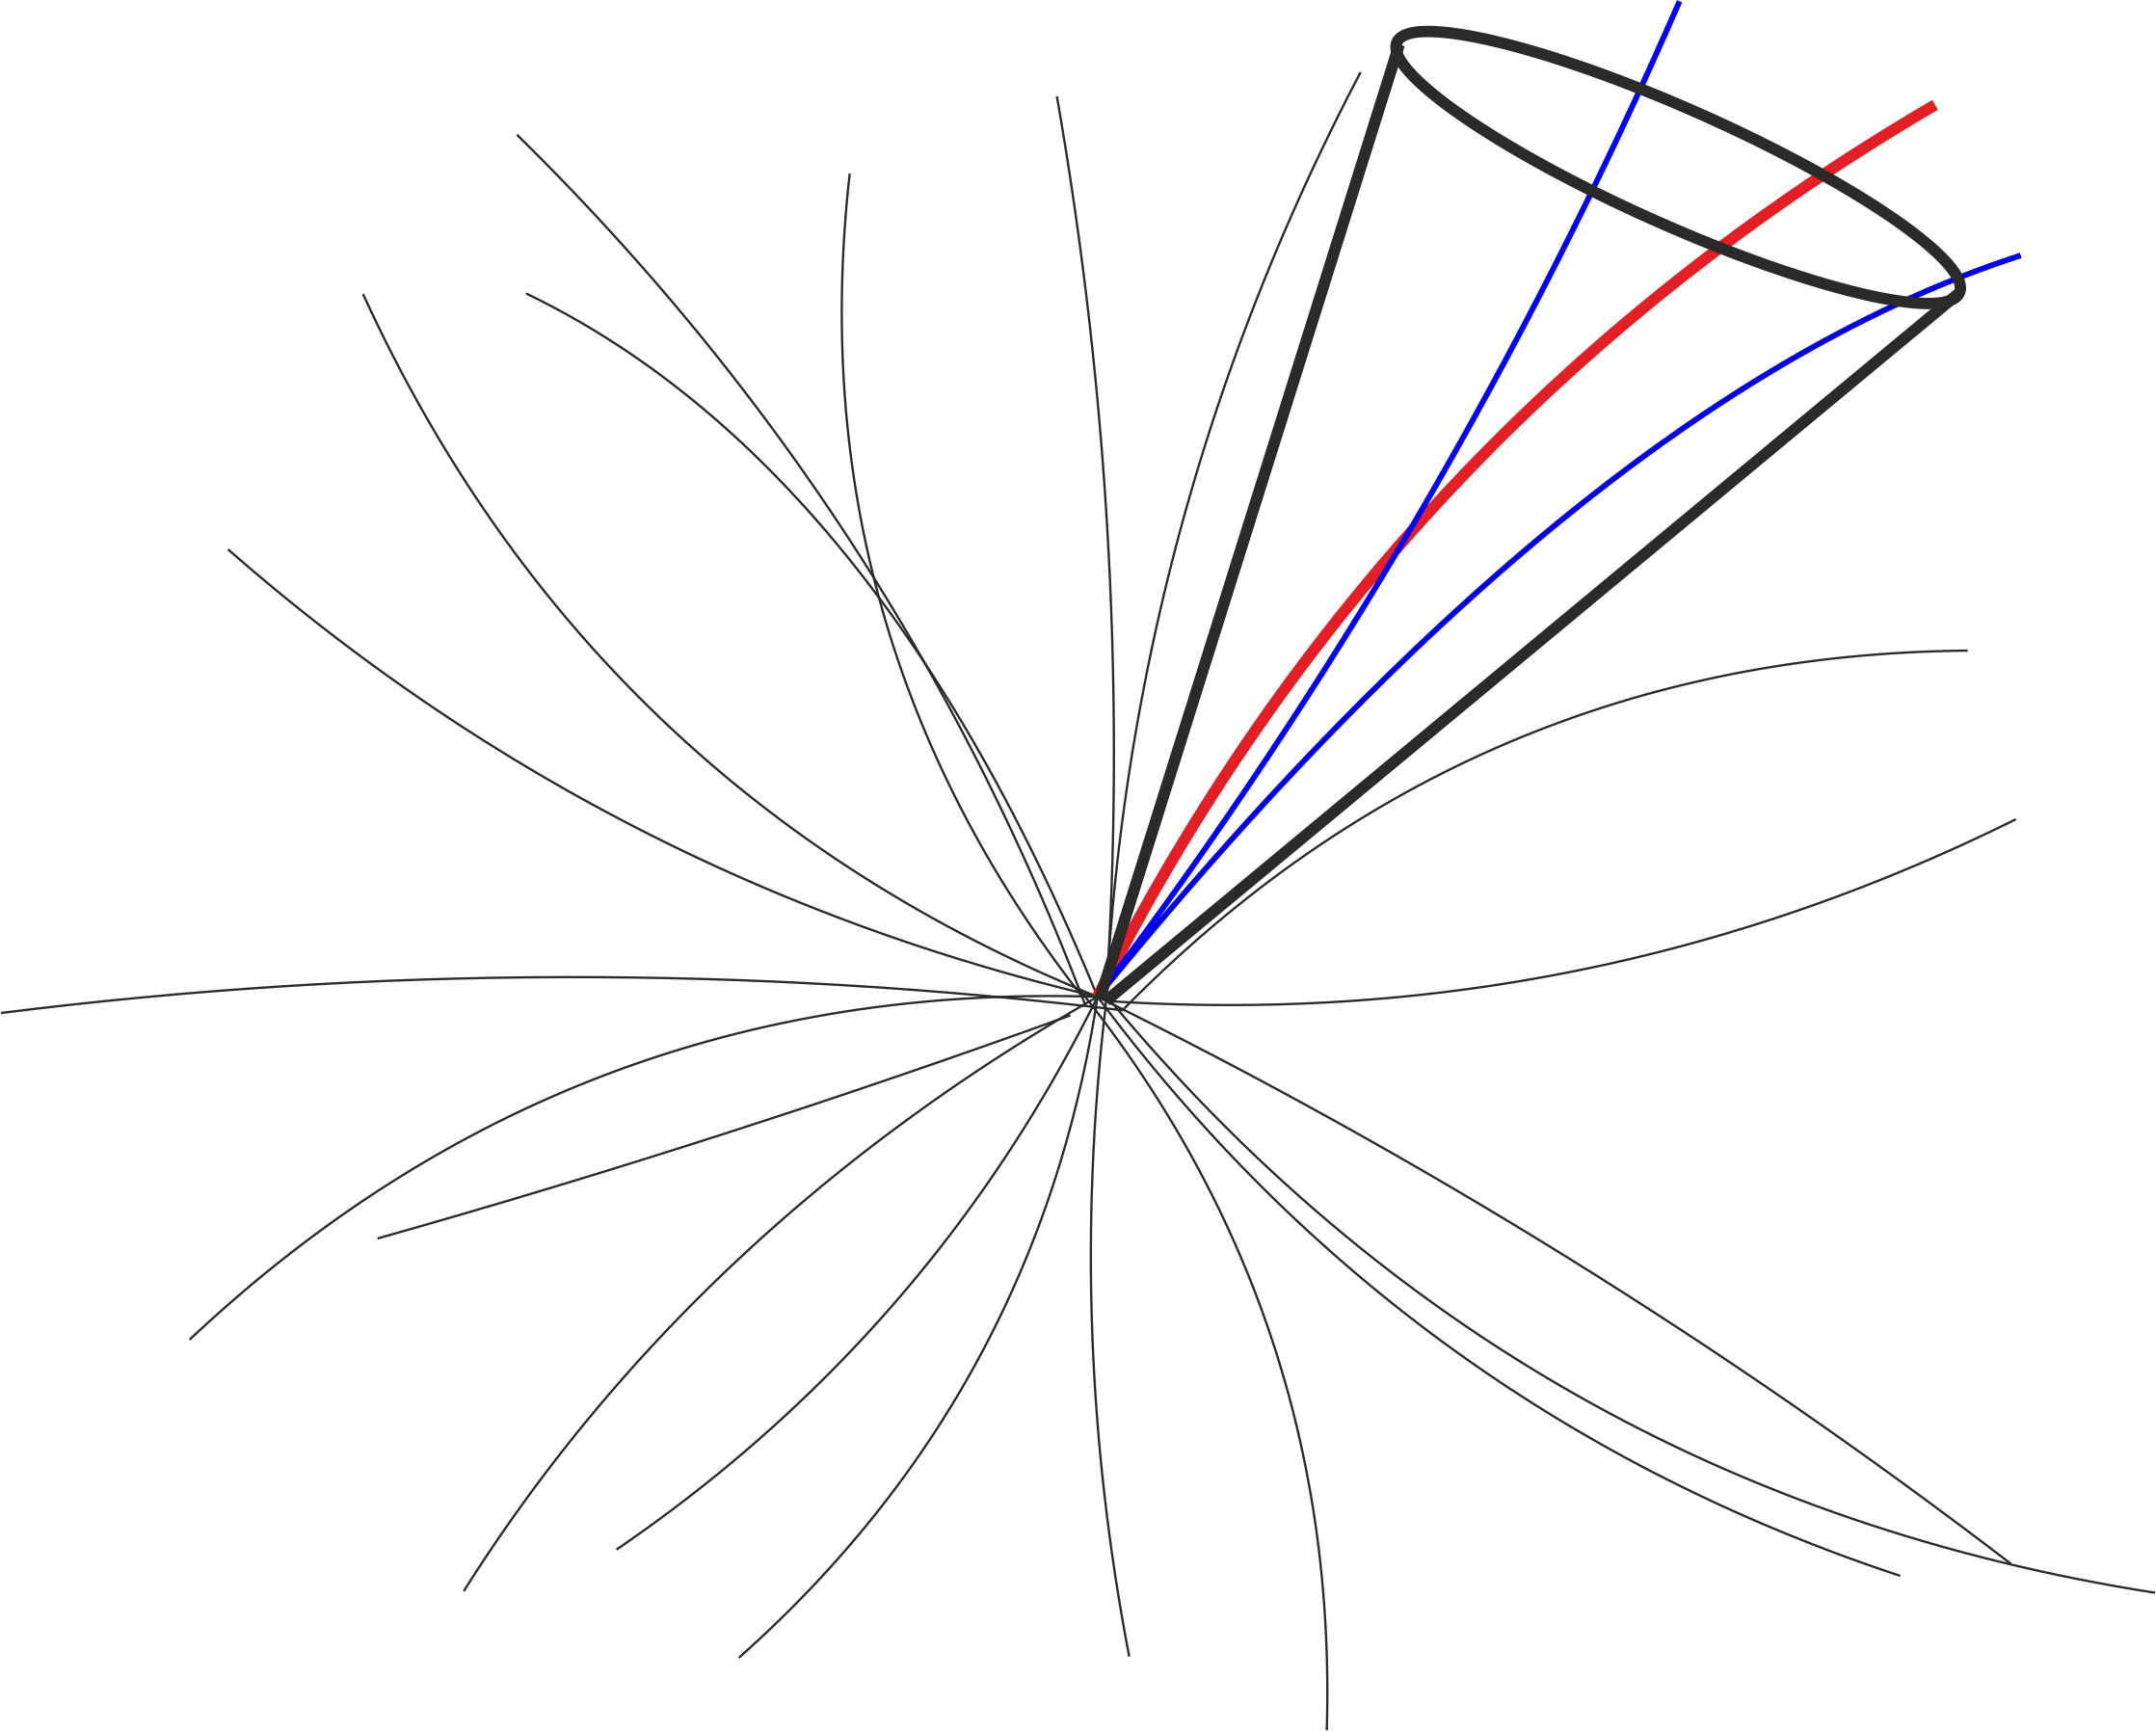
\includegraphics[width=\textwidth,valign=T]{cone}
	\end{column}
	\begin{column}{.3\textwidth}
		
		\small
		{\color{red} Hard-scattering particle} \\
		\vskip0.8cm
		{\color{cyan} Pile-up particles in RoI} \\
		\vskip0.8cm
		{\color{gray} Pile-up particles outside RoI} \\
		\vskip1.5cm
		\framebox{Cone $\Delta$R = 0.1}
	\end{column}
\end{columns}
	
\end{frame}

%----------------------------------------------

\begin{frame}[t]
\frametitle{The Fast Sim method - Algorithm}

\only<1>{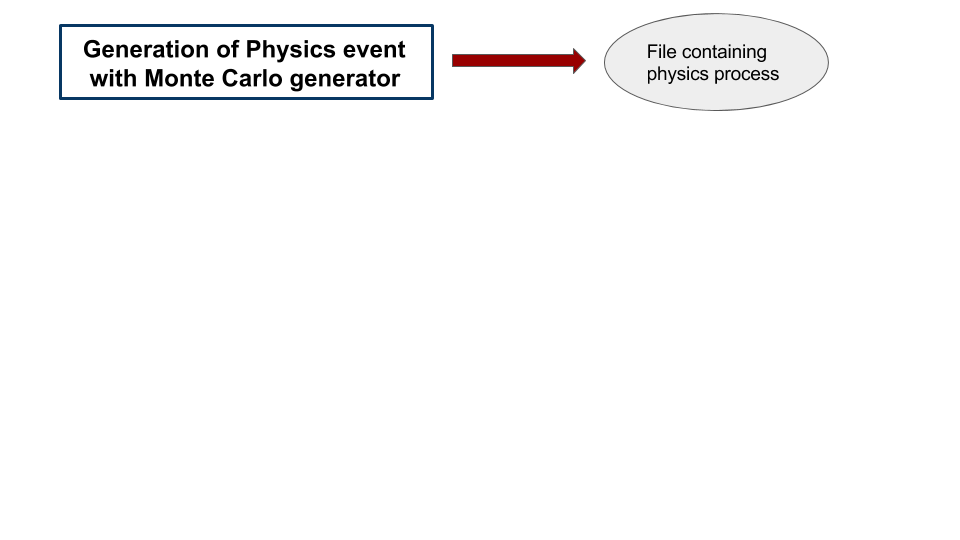
\includegraphics[width=\textwidth]{PhysicsGenerationFlow_1}}
\only<2>{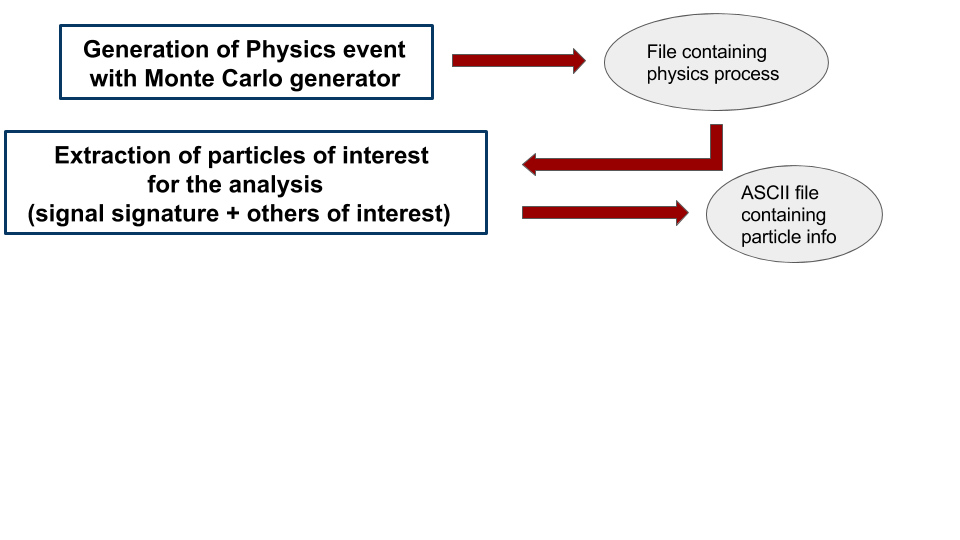
\includegraphics[width=\textwidth]{PhysicsGenerationFlow_2}}
\only<3>{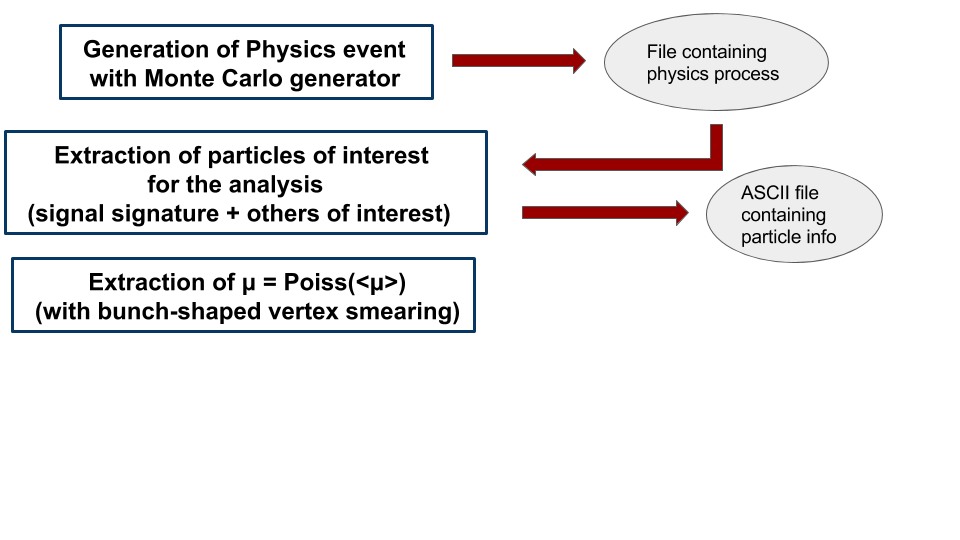
\includegraphics[width=\textwidth]{PhysicsGenerationFlow_3}}
\only<4>{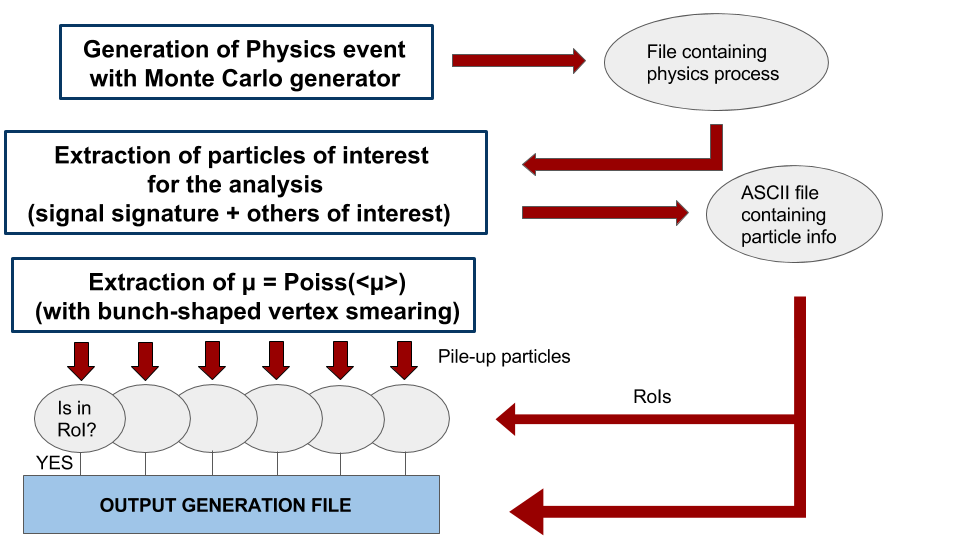
\includegraphics[width=\textwidth]{PhysicsGenerationFlow_4}}

\transdissolve<2-4>
\end{frame}

%----------------------------------------------

\begin{frame}[t]
\frametitle{Generated events}

\begin{itemize}
\item 50k events of $H \rightarrow ZZ^{*} \rightarrow 4\mu$ (signal) \tikzmark{topbrace}
\item 16k events of $ZZ^{(*)} \rightarrow 4\mu$ (background) \tikzmark{bottombrace}
\end{itemize}

\setbeamercolor{local structure}{fg=dred} 
\begin{itemize}
\item only events with exactly four muons and photons with $p_{T, max}^{\gamma} < 1.5$ GeV
\end{itemize}
%[\color{red}\scalebox{0.9}{\ball}]
\begin{tikzpicture}[overlay, remember picture]
\draw [decoration={brace,amplitude=0.5em},decorate,ultra thick,black]
let \p1=(topbrace), \p2=(bottombrace) in
({max(\x1,\x2)}, {\y1+0.8em}) -- node[right=0.6em] {POWHEG} ({max(\x1,\x2)}, {\y2});
\end{tikzpicture}
%

\begin{columns}
\begin{column}{.5\textwidth}
\centering
Truth $4\mu$ mass in $ZZ^{(*)} \rightarrow 4\mu$
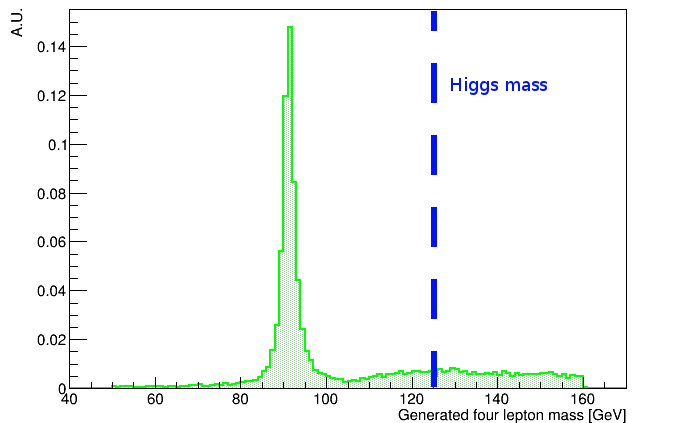
\includegraphics[width=\textwidth]{ZZ4mu/gen4muMass4}
\end{column}
\begin{column}{.5\textwidth}
\centering
Photon $p_{T}$\par
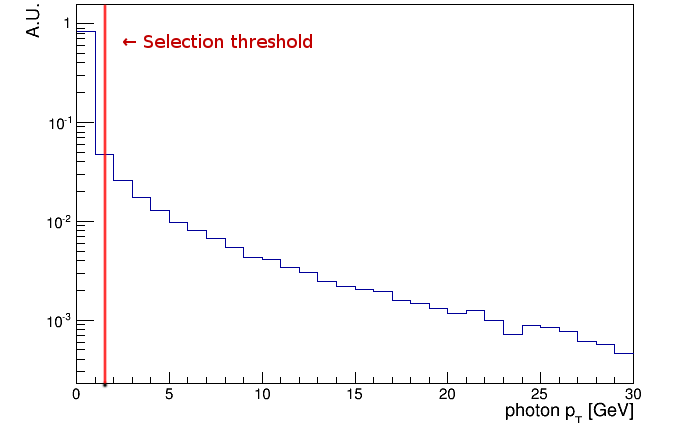
\includegraphics[width=\textwidth]{HZZ4mu/photonPt4}
\end{column}
\end{columns}
\end{frame}

%----------------------------------------------

\begin{frame}
\frametitle{Truth Z mass distribution}

\begin{columns}
\begin{column}{.5\textwidth}
\centering
$H \rightarrow ZZ^* \rightarrow 4\mu$
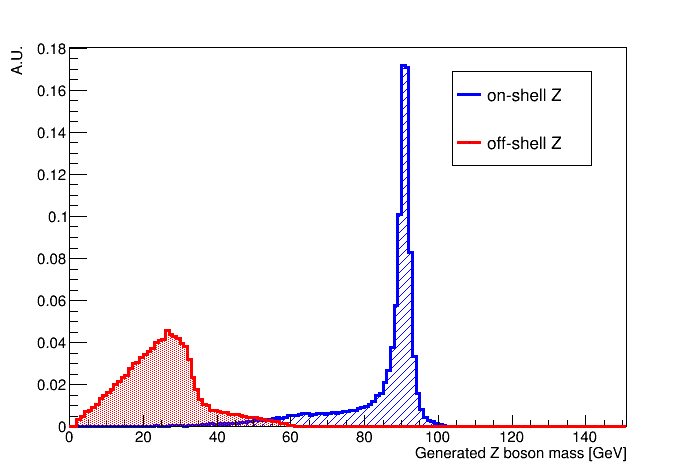
\includegraphics[width=\textwidth]{HZZ4mu/genZMass}
\end{column}
\begin{column}{.5\textwidth}
\centering
$ZZ^{(*)} \rightarrow 4\mu$\par
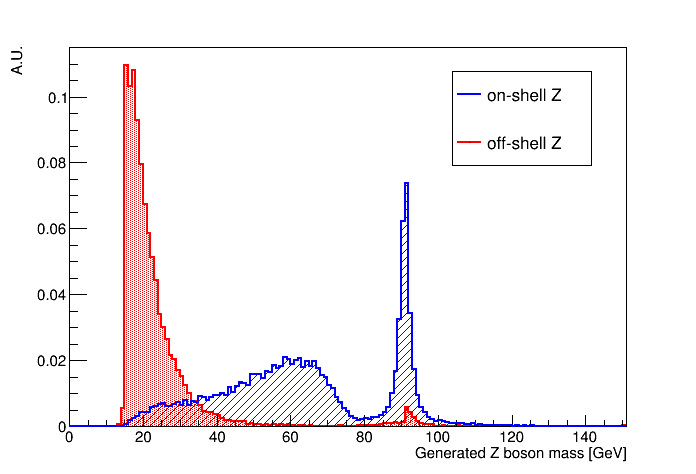
\includegraphics[width=\textwidth]{ZZ4mu/genZMass}
\end{column}
\end{columns}
\end{frame}

%----------------------------------------------

\begin{frame}[t]
\frametitle{Analysis selection}

Requirements are applied in sequence:
\begin{itemize}
\item<1-> at least four tracks in the event;
\item<2-> tracks must consist of at least 10 hits;
\item<3-> tracks must have $p_{T} >$ 6 GeV;
\item<4-> tracks should be closer than 5$\sigma_{z}$ to the truth primary vertex;
\end{itemize}
\medskip
\pause
\pause
\pause
\pause
At this point, all events contain no more than four tracks:
\begin{itemize}
\item<6-> tracks should be isolated: $\sum_{\Delta R < 0.1} (p_{T}) / p_{T, candidate} <$ 1;
\item<7-> the system must be electrically neutral;
\item<8-> the ordered $p_{T}$ of the tracks must be ($>$ 20, $>$ 15, $>$10, $>$ 6) GeV;
\item<9-> at least one of the off-shell candidates (neutral pair with most distant mass from the Z)
must lie in the region $|\eta| <$ 2.7;
\item<10-> the mass of the on-shell pair should lie in the region [50,106] GeV;
\item<11-> the mass of the off-shell pair should lie in the region [12,115] GeV;
\end{itemize}

\end{frame}

%----------------------------------------------

\begin{frame}
\frametitle{Selection efficiency}
\centering
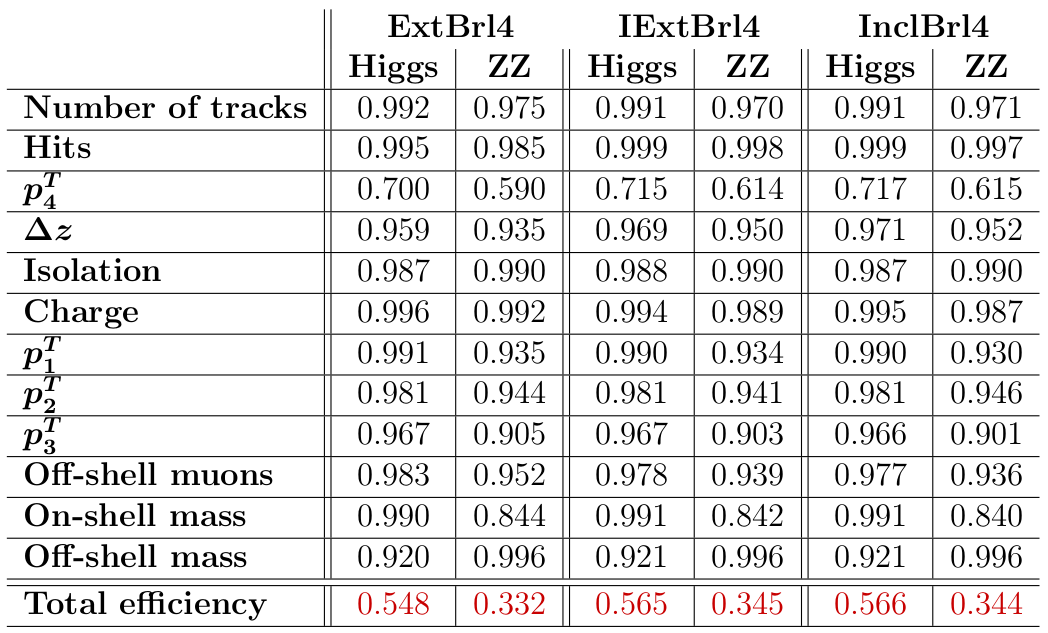
\includegraphics[width=\textwidth]{Efficiency}
\end{frame}

%----------------------------------------------

\begin{frame}[t]
\frametitle{Comparison with the Scoping Document}
\begin{columns}
\begin{column}{.6\textwidth}
\centering
Scoping Document: Efficiency (InclBrl4)
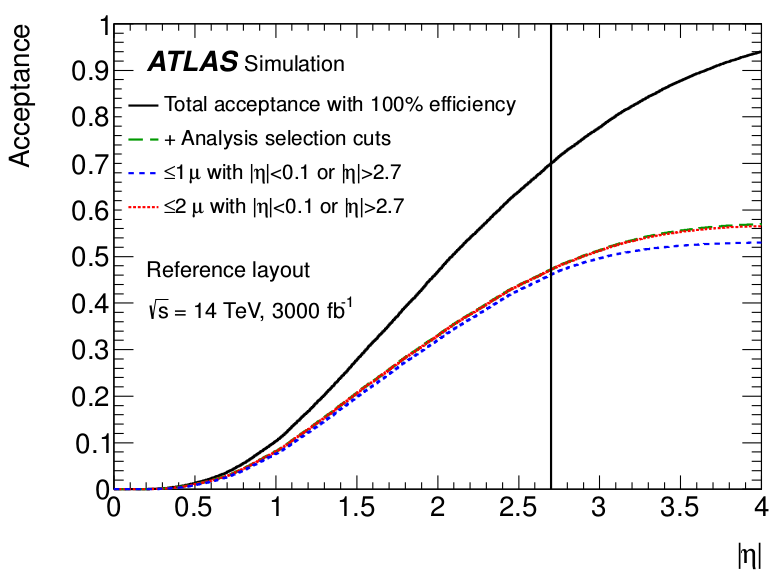
\includegraphics[width=\textwidth]{scopingAcceptance}
\end{column}
\begin{column}{.4\textwidth}
\resizebox{\textwidth}{!}{
\begin{tabular}{|c|c|c|}
\hline
 & \textbf{Us} & \textbf{Scoping} \\ \hline
\textbf{Geom. acc.} & 94.08\% & 94\% \\ \hline
\textbf{Total eff.} & 56.6\% & 57\% \\ \hline
\end{tabular}}
\end{column}
\end{columns}

\medskip
\begin{center}
\framebox{\color{dred} Very compatible results, but different layouts}
\end{center}
\end{frame}

%----------------------------------------------

\begin{frame}[t]
\frametitle{On-shell mass resolution}

\begin{columns}
\begin{column}{.5\textwidth}
\centering
\vskip1.2cm
Scoping Document
\includegraphics<1>[width=\textwidth,height=4.5cm]{scopingSigOnShell27}
\includegraphics<2>[width=\textwidth,height=4.5cm]{scopingSigOnShell32}
\includegraphics<3>[width=\textwidth,height=4.5cm]{scopingSigOnShell4}
\end{column}
\begin{column}{.5\textwidth}
\centering
\vskip1.0cm
Our analysis (InclBrl4 layout)
\vskip0.1cm
\includegraphics<1>[width=\textwidth]{HZZ4mu/recoOnShellMass27}
\includegraphics<2>[width=\textwidth]{HZZ4mu/recoOnShellMass32}
\includegraphics<3>[width=\textwidth]{HZZ4mu/recoOnShellMass4}
\end{column}

\end{columns}
\end{frame}

%----------------------------------------------

\begin{frame}[t]
\frametitle{$4\mu$ mass resolution}

\begin{columns}
\begin{column}{.5\textwidth}
\centering
\vskip1.2cm
Scoping Document
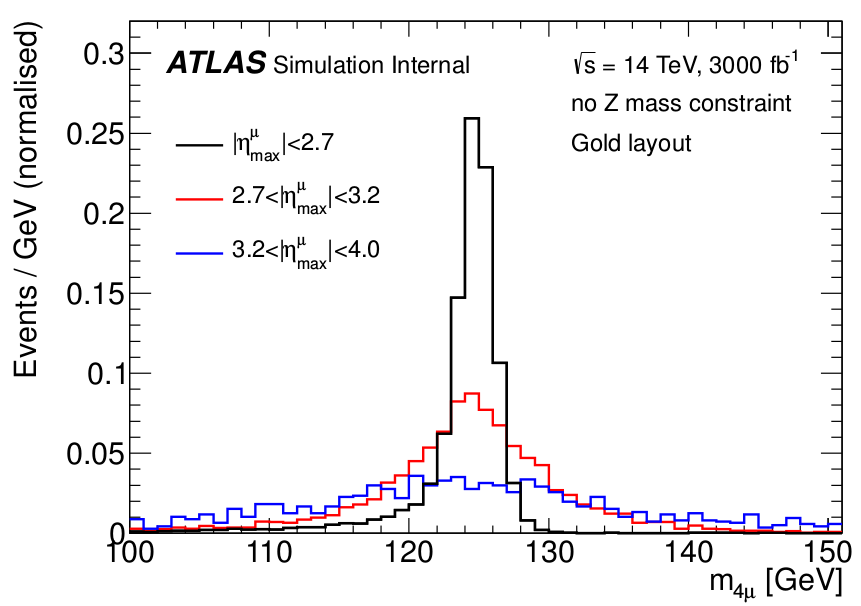
\includegraphics[width=\textwidth]{scopingRecoMass}
\end{column}
\begin{column}{.5\textwidth}
\centering
\vskip1.2cm
Our analysis (InclBrl4 layout)
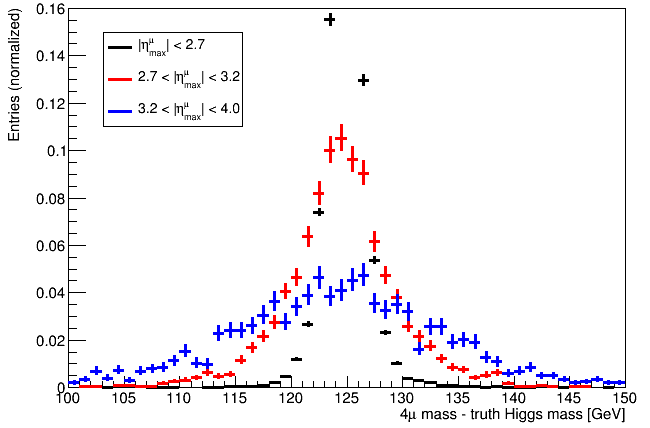
\includegraphics[width=\textwidth]{HZZ4mu/recoMass}
\end{column}

\end{columns}
\end{frame}

%----------------------------------------------

\begin{frame}
\frametitle{Higgs $p_{T}$, $\eta$, $\phi$ resolutions}
\begin{columns}
\begin{column}{0.5\textwidth}
\centering
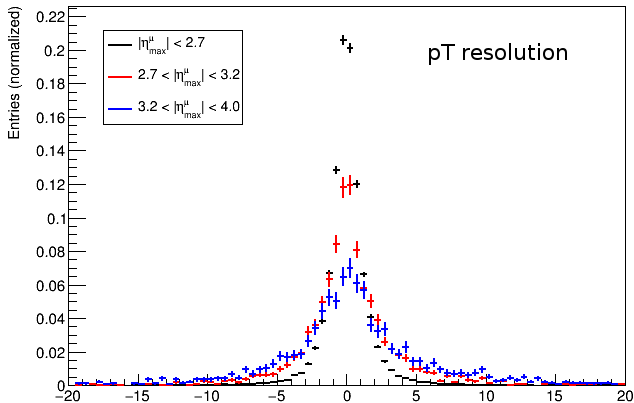
\includegraphics[width=\textwidth,height=3.7cm]{HZZ4mu/sigRecoPt}
\end{column}
\begin{column}{0.5\textwidth}
\centering
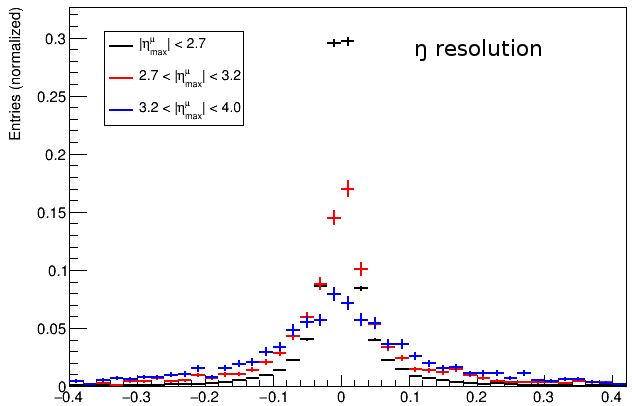
\includegraphics[width=\textwidth,height=3.7cm]{HZZ4mu/sigRecoEta}
\end{column}
\end{columns}
\vskip-0.5cm
\begin{center}
\centering
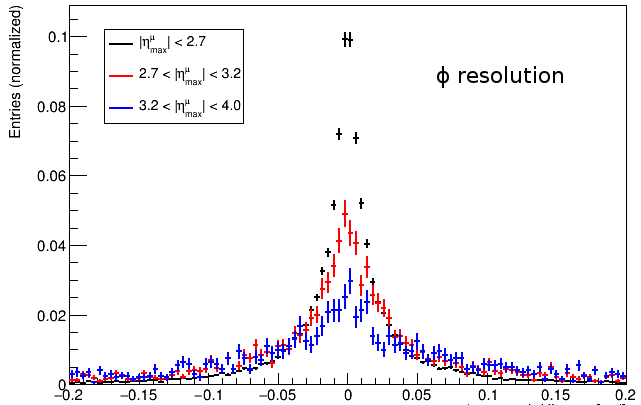
\includegraphics[width=0.5\textwidth,height=3.7cm]{HZZ4mu/sigRecoPhi}
\end{center}

\end{frame}


%----------------------------------------------

\begin{frame}
\frametitle{Muon $p_{T}$, $\eta$, $\phi$ resolutions}
\begin{columns}
\begin{column}{0.5\textwidth}
\centering
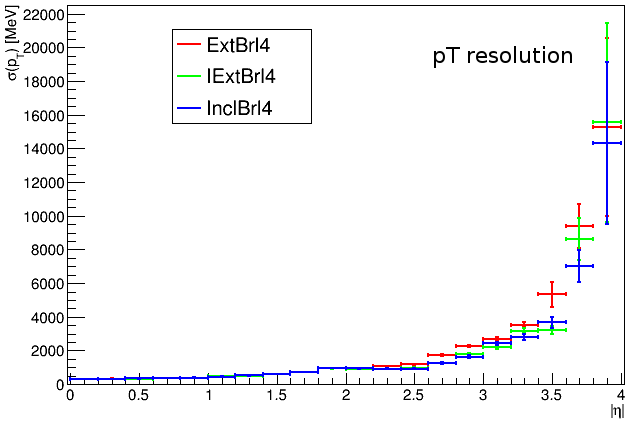
\includegraphics[width=\textwidth,height=3.7cm]{sigPt}
\end{column}
\begin{column}{0.5\textwidth}
\centering
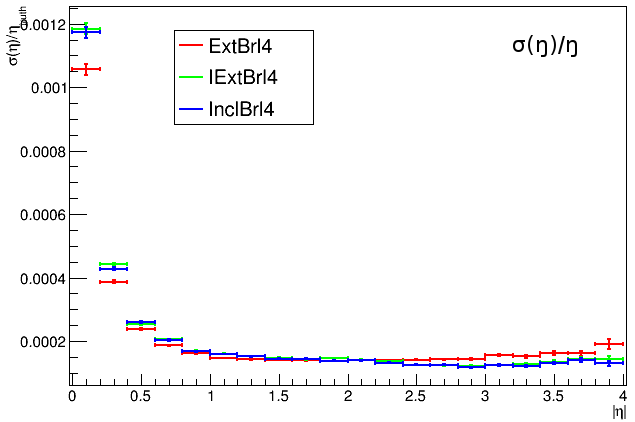
\includegraphics[width=\textwidth,height=3.7cm]{sigEta}
\end{column}
\end{columns}
\vskip-0.5cm
\begin{center}
\centering
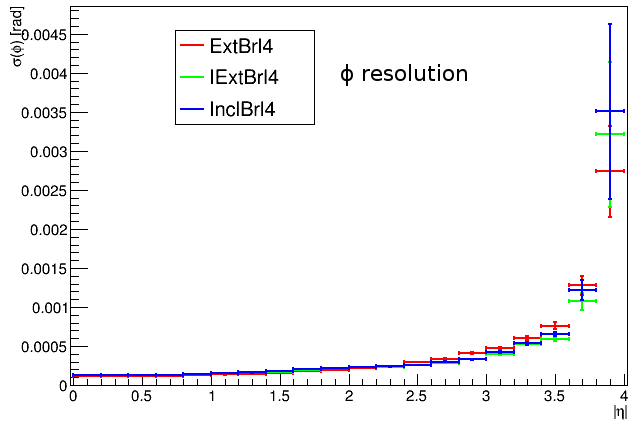
\includegraphics[width=0.5\textwidth,height=3.7cm]{sigPhi}
\end{center}

\end{frame}

%----------------------------------------------

\begin{frame}
\centering
\huge \color{dred} \textbf{Backup slides}
\end{frame}

\begin{frame}
\frametitle{Layouts}
\begin{columns}
\begin{column}{0.5\textwidth}
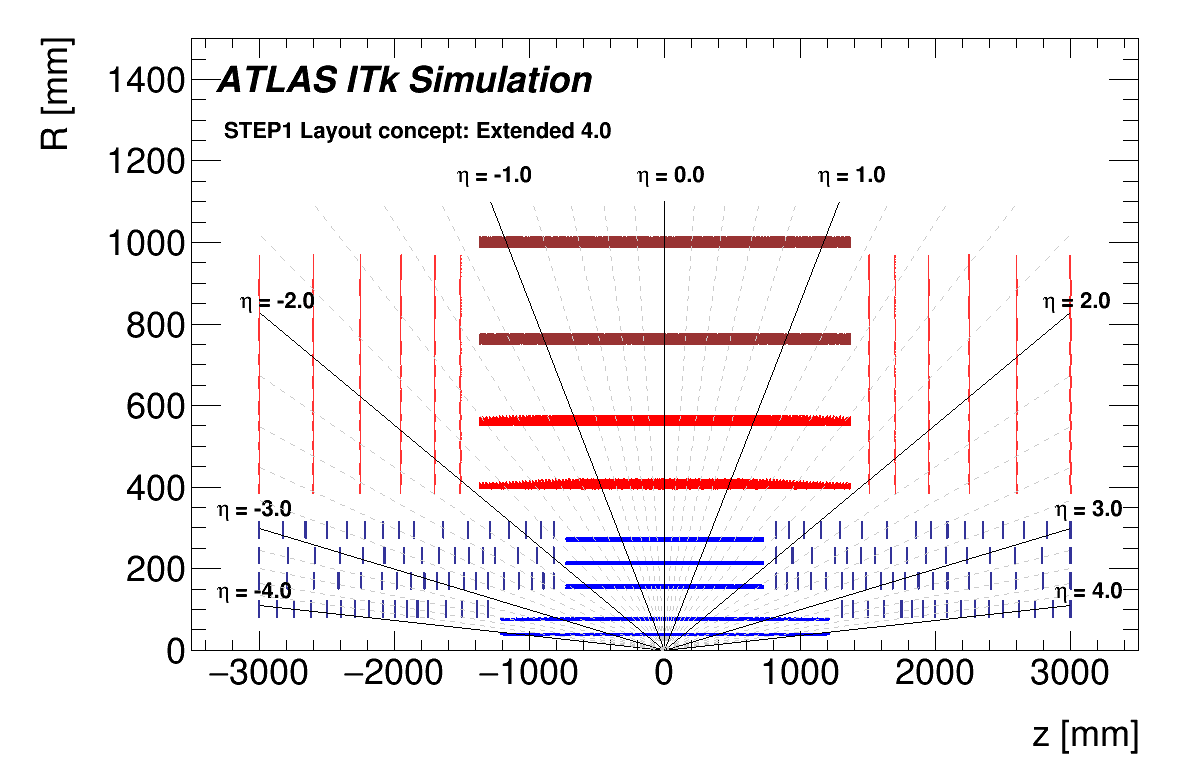
\includegraphics[width=\textwidth,height=3.8cm]{ExtBrl4}
\end{column}
\begin{column}{0.5\textwidth}
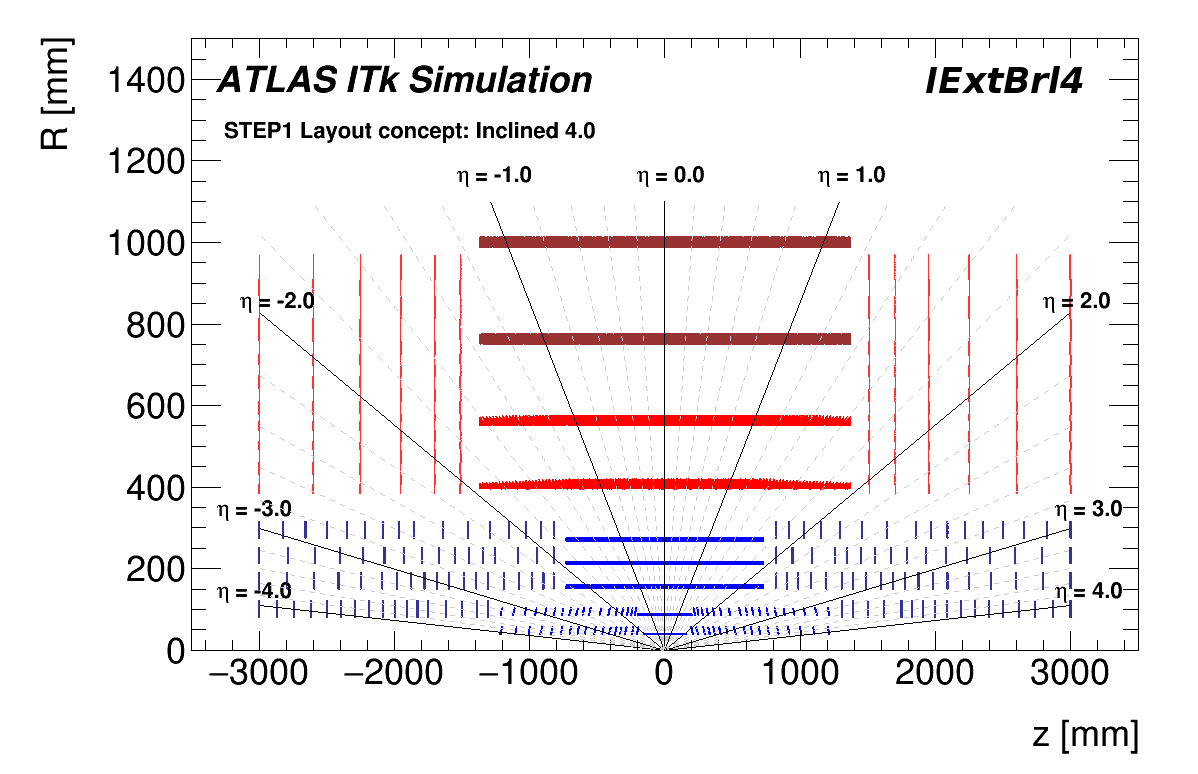
\includegraphics[width=\textwidth,height=3.8cm]{IExtBrl4}
\end{column}
\end{columns}

\begin{center}
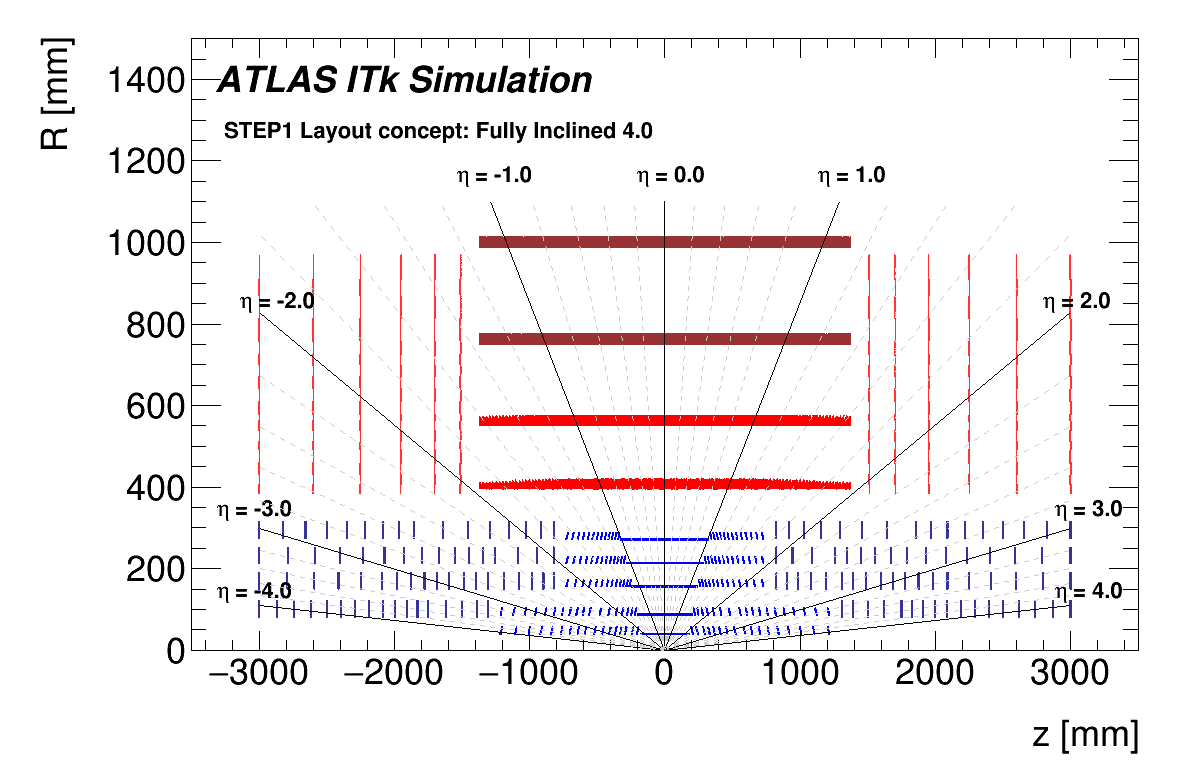
\includegraphics[width=0.5\textwidth,height=3.8cm]{InclBrl4}
\end{center}

\end{frame}

\end{document}